


Since the inception of attosecond streaking \cite{Zenghu2005,KellerAngularStreaking} there have been great recent gains in diagnosing euv pulses that encroach on the soft x-ray regime \cite{Biegert2016,WornerSci2017,Worner2017}.
Some phase retrieval analysis require interferences with reference oscillators as in Refs.~\cite{Zenghu2010,Cocke2013}, we favor a more flexible scheme that can also accommodate \textit{in situ} x-ray experiments as well as the pulse retrieval diagnostic.
We will therefore focus on the angular array of electron spectrometers as used for our recend proof of concept in Ref.~\cite{Nick2018}.



There is increasing momentum in the development of spectro-temporally shaped x-ray FEL pulses \cite{eehg2009,Lutman13_twocolor,Marinelli13_twocolor,Allaria2014,Marinelli2015,Hemsing2016,Prince2016,Lutman2016,Marinelli2016} in response to the rising tide of demand \cite{Mukamel2007,Biggs2012,Mukamel2013,4WaveMixing,TIGER2015}.
The predominant method to characterize such novel temporal profiles is based on an x-band transverse accelerating cavity (XTCAV) \cite{xtcav2014} whereby the spent electron bunch is deflected horizontally, streaked in time by the phase of the transverse accelerating field.
A bending magnet then deflects this time-streaked beam vertically proportional to the energy.
Imaging the result, one records the time-energy distribution of the spent bunch.
This technique has been a critical tool for developing the recent x-ray FEL pulse shaping methods \cite{Marinelli2015,Marinelli2016}.
Unfortunately, it indirectly measures the x-ray temporal profile by identifying the imprint of lasing on the electron bunch.
Furthermore, barring a superconducting upgrade to the x-band cavity, the XTCAV can only run at 120 Hz.

\begin{wrapfigure}[10]{r}{.5\linewidth}
\vspace{-\baselineskip}
\centerline{
	%\includegraphics[trim = {-2cm -2cm 2cm 1.7cm},clip,height=7.5cm]{newstreaking.cartoon.new.eps}
	\includegraphics[width=\linewidth]{naturePhoton_NickWolfi.clockfig.eps}
}
\vspace{-\baselineskip}
\caption{
	\label{streakingschematic} 
	Schematic of angular photo-electron streaking. \cite{Nick1028}
}
\end{wrapfigure}

Photo-electron streaking, a direct interaction, has the capability to measure the instantaneous temporal structure of x-ray pulses \cite{Hentschel2001}.
In photo-electron streaking, a noble gas like neon is dressed by a strong far-infrared or THz field \cite{Helml2014,Juranic2014,Schulz2015}.
As depicted in Fig.~\ref{streakingschematic}, the vector potential of the streaking field shifts the outgoing photo-electron energy depending on the phase of the field at the time of photoionization.
The temporal shape (purple) can then be read out by the intensity profile of the photo-electrons versus their shifted energies (green), given that the pulse arrives near the zero-crossing of the vector potential.
Our recent use of the organic crystal DAST \cite{DAST} for THz generation was capable of resolving 50 fs separated double pulses of the LCLS \cite{Matthias2016} that Cavalieri\etal have developed into robust photo-electron streaking system \cite{Schulz2015}.
Such THz and far infrared based schemes \cite{Helml2014,Juranic2014} have a demanding $\sim$2 mJ/pulse laser power requirement will likely not scale well for the high repetition rates of LCLS-II (Table~\ref{lcls2specs}).

The requirement that the x-ray pulse arrive near a zero-crossing of the vector potential is a persistent challenge.
The Cavalieri group creatively arranges two photo-electron spectrometers to sample the focal volume of the THz field at two different places across the Gouy phase of the focus.
As a beam propagates through a focus it develops a phase advance of $\pi$ --- the Gouy phase --- such that one can choose two points just on either side of the focus that have a $\pi$/2 Gouy phase difference.
For shots when one of the detectors records the zero crossing of the field, the other detector will measure the maximum kick, thus calibrating the zero-crossing slope.
In practice, however, THz and mid-infrared fields depend rather sensitively on environmental factors and on exactly from where in the Gouy phase one measures these streaked photo-electrons.
Juranic\etal have attempted to use three spectrometers, one for the unstreaked photo-electron spectrum, and two back-to-back spectrometers to record simultaneously the positively and negatively streaked spectra.
This method still suffers when the pulse arrives sufficiently away from the optimal zero-crossing phase.




Miscalibration of the streaking ramp is also common since the changing particulars of the experiment, such as humidity and pump pointing, can dramatically affect the exact shape of the streaking field.
%The fragility of the carrier field to environmental fluctuations scales with the fractional bandwidth ($\Delta\omega/\omega_0$) used to support the pulse duration.
For the single cycle THz and few-cycle far-infrared fields typically used in x-ray streaking diagnostics, the fractional bandwidth $\Delta\omega/\omega_0$ is often nearly equal to unity.
Such extreme fractional bandwidths make for very irregular carrier fields that vary depending on beam pointing and atmospheric humidity.
%As a result, an often invasive recalibration procedure must be repeated periodically.
This is largely why we have chosen to pursue an alternative approach in Ref.~\cite{Nick2016}.

\begin{wrapfigure}[15]{r}{.5\linewidth}
%\centerline{\includegraphics[trim = {0 1cm 0 1cm},clip,width=\linewidth]{NickSchemeAngularStreaking.eps}}
\vspace{-.5\baselineskip}
\caption{\label{NickScheme}
Angular streaking schematic.
}
\end{wrapfigure}

We will leverage our long history with photo-electron streaking at the LCLS \cite{Duesterer11,Meyer12,Helml2014} by extending the attosecond angular streaking method of Refs.~\cite{CorkumAngularStreaking,KellerAngularStreaking} to the x-ray regime.
Pulse-to-pulse variations at an FEL require single-shot measurements much like the velocity map imaging (VMI) \cite{VrakkingRSI} extension of attosecond angular streaking \cite{attoclockVMI2013}.
The requirement of a two-dimensional detector, however, likely precludes high repetition rates. 
We will therefore repurpose what is more traditionally considered an x-ray FEL polarimeter \cite{Markus2014,Allaria2014,Mazza2014,Lutman2016} to measure the angularly streaked photo-electron spectra \cite{Markus2014,Allaria2014,Mazza2014,Lutman2016}.

We recently demonstrated attosecond angular streaking at LCLS with an angular array of 16 electron time-of-flight detectors --- the ``CookieBox'' --- as depicted in Fig.~\ref{NickScheme}.
We measured full photo-electron spectra in each of the 16 detectors operating in current, not counting, mode.
The result was an x-ray pulse temporal reconstruction with 500 attoseconds resolution \cite{Nick2016} which we propose here to extend to the 150 attoseconds resolution scale.
We also plan to demonstrate both spectral and polarization sensitivity versus time as well as operation at high repetition rate.

\begin{wrapfigure}[20]{l}{.5\linewidth}
\vspace{-\baselineskip}
%\centerline{\includegraphics[trim = {0cm 0 18.5cm 0},clip,width=\linewidth]{nick_fig2.eps}}
%\centerline{\includegraphics[trim = {18.5cm 0 0 0},clip,width=\linewidth]{nick_fig2.eps}}
\vspace{-1\baselineskip}
\caption{\label{NickRetrieval}X-ray pulse shape retrieval from our recent angular streaking measurement at LCLS \cite{Nick2016}.}
\end{wrapfigure}

In angular streaking, the x-ray pulse produces neon photo-electrons that distribute into a dipole probability distribution with a common kinetic energy regardless of emission angle.
When dressed with the circularly polarized laser field, shown as the red corkscrew pattern in Fig.~\ref{NickScheme}, those electrons will receive a momentum kick toward the instantaneous direction of the vector potential in a reference frame that spirals relative to the lab frame at the carrier cycle frequency.
In this way, one detector will measure electrons with an excess of energy, the opposite detector with less energy, and the two orthogonal detectors will measure the photo-electrons as the projected vector-potential sweeps through a zero-crossing.
The additional detectors further constrain the pulse shape retrieval shown in Fig.~\ref{NickRetrieval} where the measured spectra reveal a nearly single sub-fs FEL pulse as required for such techniques as impulsive x-ray Raman spectroscopy \cite{TIGER2015}.

Preliminary results demonstrate 500 attoseconds resolution \cite{Nick2016}.
This resolution depends both on the spectral resolution of the electron time-of-flight spectrometers and on the number of angular sample points per optical cycle.
The typical space constraints near beamlines and individual detector geometries limits the CookieBox array to 16 detectors. %a 1 meter diameter by limiting the number of detectors.
%The diminishing returns for adding more detector assemblies has driven the design to 16 angles.
Modeled after the original Viefhaus design, we propose a universal main chamber that can accept a micro-channel plate based electron detector with 100 ps impulse response.
We have begun discussions with the detector group at University of Bern regarding the design of a modular CookieBox style system.
Of particular interest is the application of super-resolution concepts, such as explored for temporal sorting in Objective~\ref{obj::sorting}.
One generally seeks a non-uniformly distributed under-sampling of a waveform, in this case the angular distribution, in order to reconstruct an accurately interpolated result \cite{Candes2004a,Candes2004b,Candes2005,Elad2006}. 
In simulation we will explore the efficacy of non-uniformly placed detectors for super-resolution in the angular distribution.

We will also shift the dressing laser frequency toward the near-infrared to improve the temporal resolution.
Based on Refs.~\cite{lcls2_opportunities,Biggs2012,Mukamel2013} we expect that much of the x-ray pulse characterization needs will lie in the sub-10 fs regime.
We propose therefore to shift to a 3 $\mu$m wavelength to both improve the fractional bandwidth for a robust carrier shape and to improve the temporal resolution while still preserving an appropriate window for pulse shape retrieval.
We expect this change to take our initial demonstration of 500 attosecond resolution for a 10 $\mu$m angular streaking field --- 33 fs optical cycle --- to an expected 150 attoseconds resolution for a 3 $\mu$m field --- 11 fs optical cycle.

More generally, the angular streaking technique can provide users with a direct measure of novel x-ray pulse shapes as required for stimulated RIXS and other multi-dimensional x-ray spectroscopic techniques \cite{Biggs2012,Mukamel2013,4WaveMixing}.
Shown in Fig.~\ref{coffeestains} we see a simulation of two xFEL pulses, one lower photon energy pulse that is linearly polarized along the horizontal and another higher photon energy pulse that is circularly polarized.
From left to right the inter-pulse delay changes from 0 fs -- 2 fs.
Such a temporal diagnostic will allow not only the demonstration of attosecond FEL pulses but also the full temporal, spectral, and polarization characterization of shaped multi-pulses.

%\begin{wrapfigure}[14]{r}{.6\linewidth}
\begin{figure}[b]
\vspace{-1.5\baselineskip}
\centerline{
%\includegraphics[trim={2cm -6cm 3cm 6cm},clip,height=.33\linewidth]{delay0.eps}
%\includegraphics[trim={2cm -6cm 3cm 6cm},clip,height=.33\linewidth]{delay-1.5.eps}
%\includegraphics[trim={0cm -2cm 0cm 2cm},clip,height=6cm]{fromNick/angular_streaking_sim_combined.reverse.eps}
}
\vspace{-1.0\baselineskip}
\caption{\label{coffeestains} Simulated 3 $\mu$m angular streaking as described in the text. From left to right, the inter-pulse delay progresses from 0 fs -- 2 fs.}
%\end{wrapfigure}
\end{figure}


\paragraph{Two-color}
Upon turn on in spring 2020, according to Fig.~\ref{fig::sxu_K}, we can run the copper linac beam into the soft x-ray undulators (SXU) and use a 4 GeV electron beam with two undulator gap settings for K values at 2 and 5 so that we can have two color operation at 300 eV and 600 eV. 
Since in this mode the energy separation between the two colors is dependent primarily on the undulator configuration, the tests performed with the copper linac are expected to extend to the superconducting linac when it comes available for testing later in calendar 2020.

\begin{wrapfigure}[27]{l}{.5\linewidth}
\centerline{
	%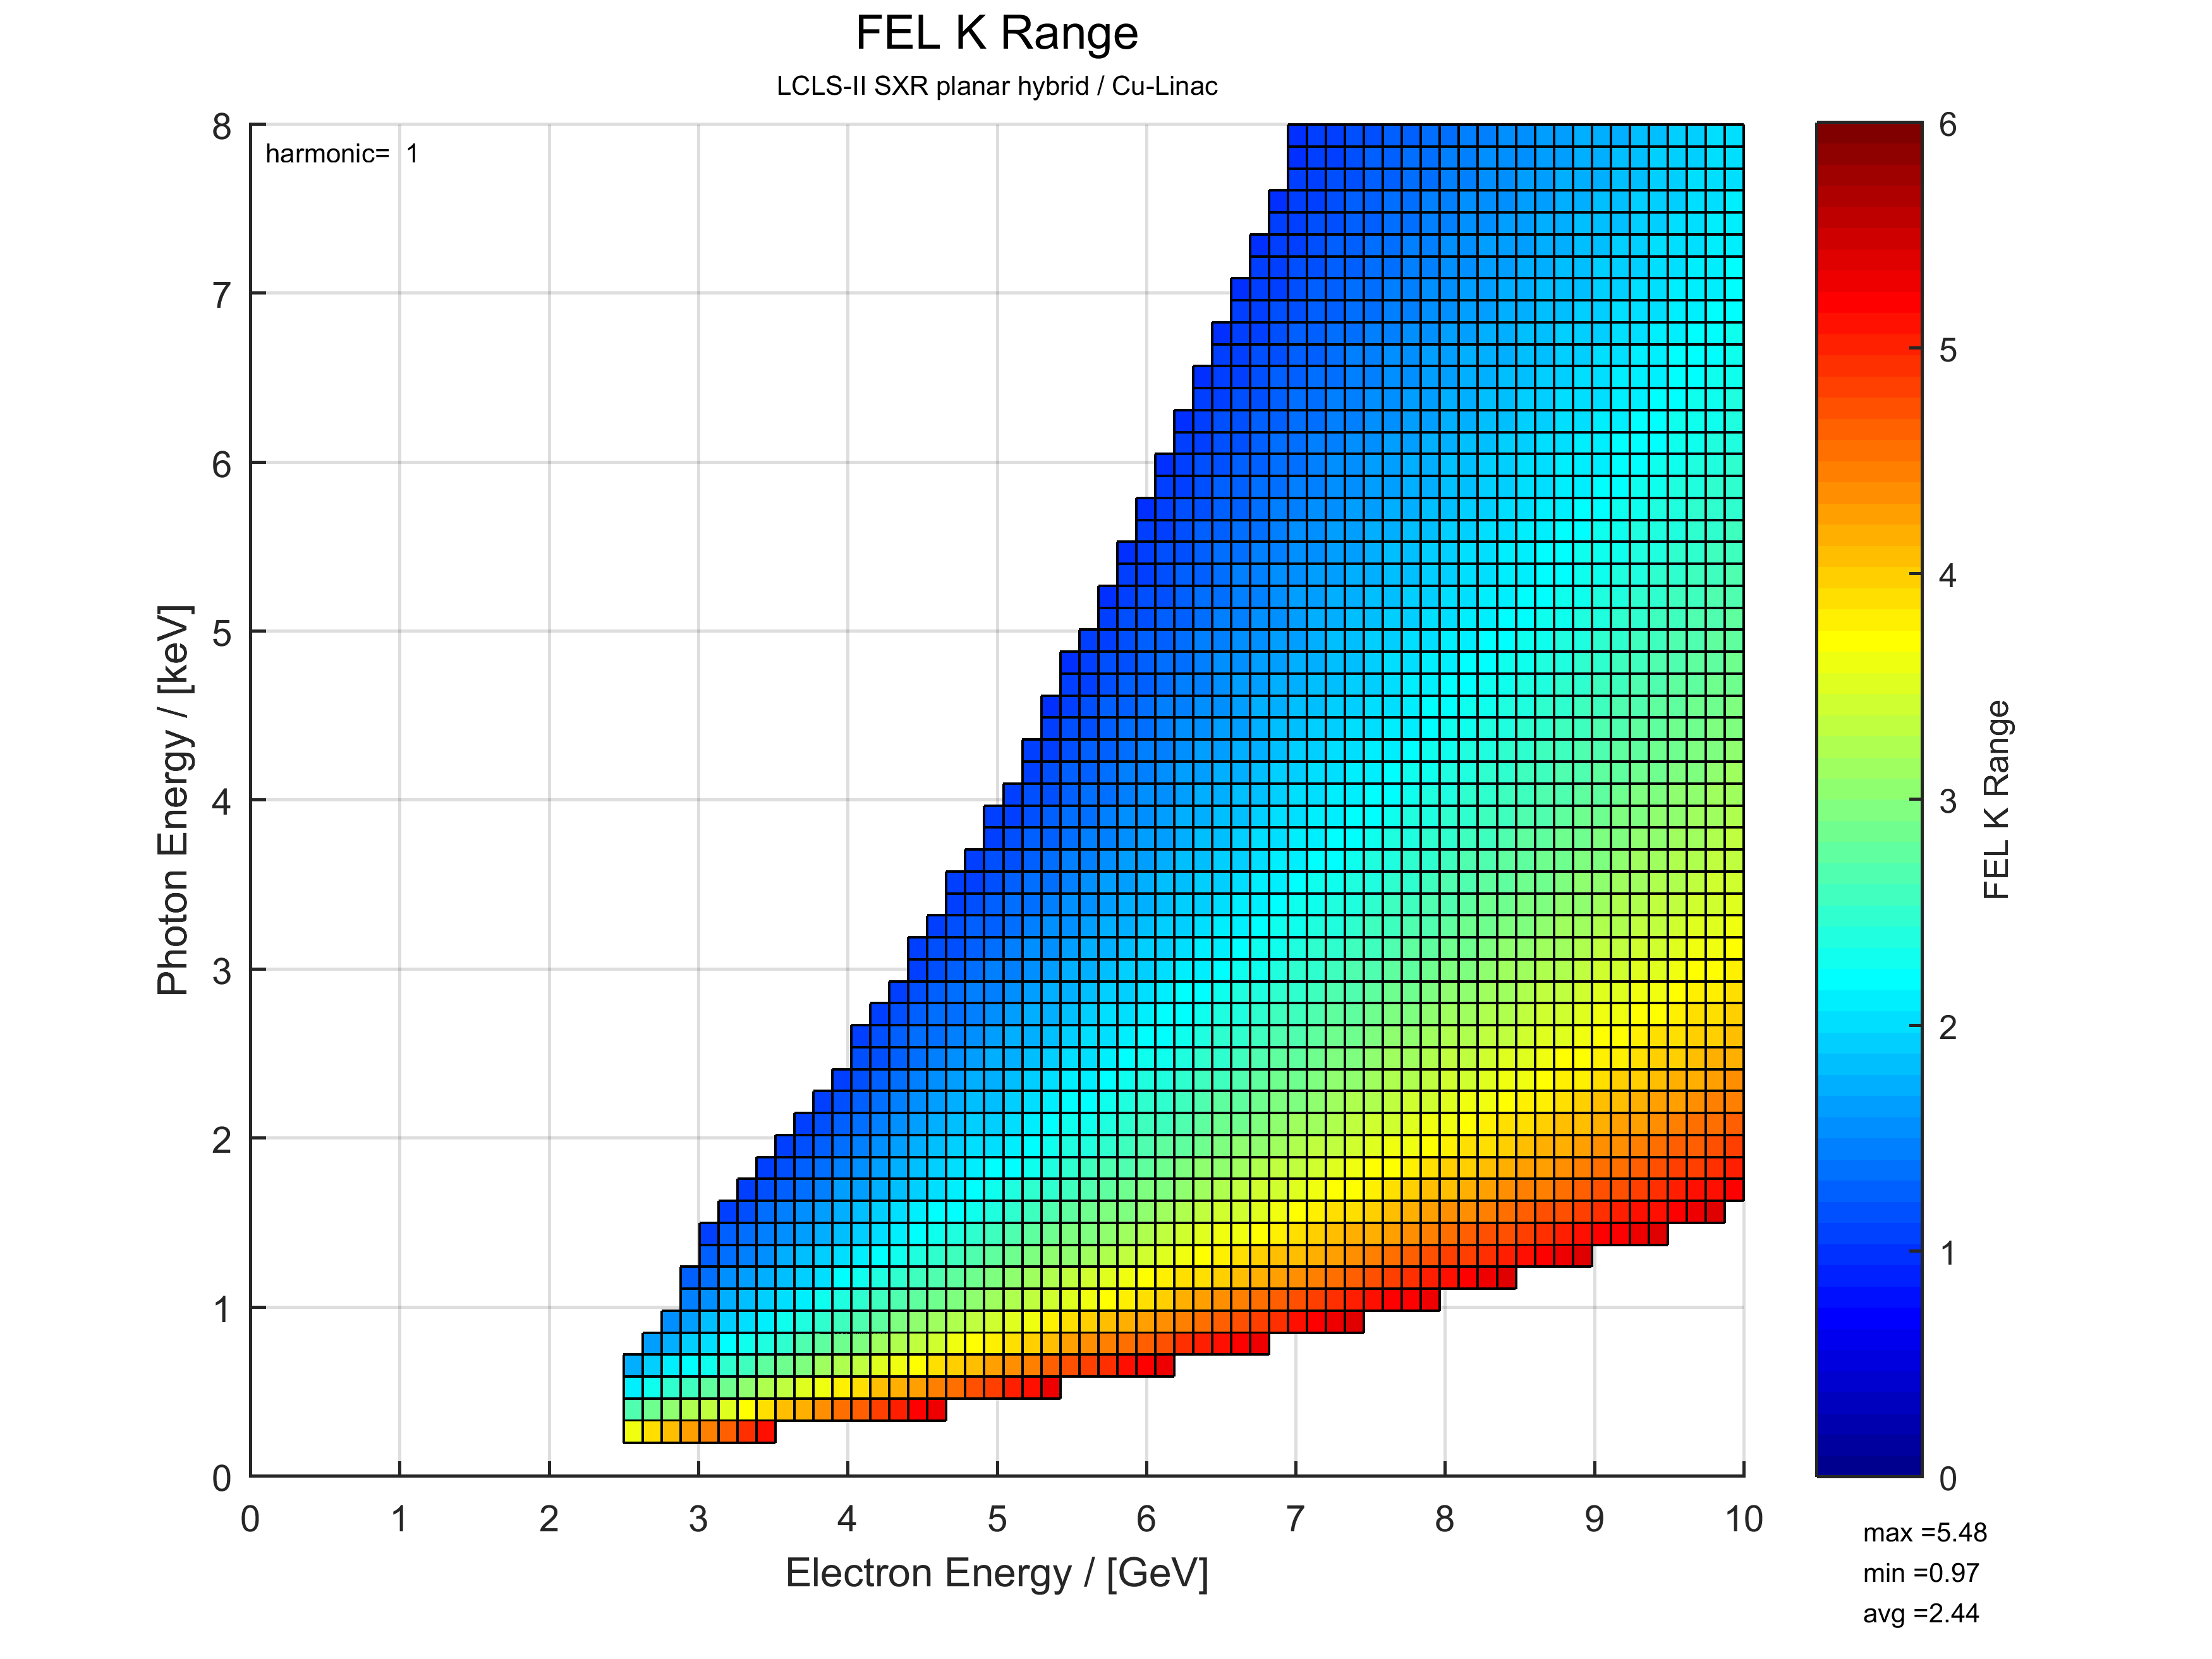
\includegraphics[width=\linewidth]{CuL_SXR_HorzPolPlanHybrid_K.eps}
	\includegraphics[width=\linewidth]{HeinzDieter_lcls2_SXU_range_lcls-tn-18-4.rangeFig.eps}
	}
	\caption{\label{fig::sxu_K} Soft x-ray undulator tuning range. \cite{HeinzDieter_SXU_twocolor,}
		}
\end{wrapfigure}
